% ==========================================================================
%  The real McCoy  --  the ideal op-amp, eleven ways a real one falls short of it, and one fix,
%  on one 16:9 landscape poster. The circuits are on opamp-circuits.tex; both \input preamble.tex.
%  Compile: just
% ==========================================================================
\RequirePackage{fix-cm}
\documentclass{article}
\usepackage[paperwidth=1067mm,paperheight=600mm,left=13mm,right=13mm,top=8mm,bottom=10mm]{geometry}
% ==========================================================================
%  Shared preamble for the op-amp slides (packages, palette, boxes, plot styles).
%  The top files set \documentclass and geometry, then \input this.
% ==========================================================================
\usepackage[utf8]{inputenc}
\usepackage[T1]{fontenc}
\usepackage[sc]{mathpazo}          % Palatino text + math
\linespread{1.05}
\usepackage{amsmath,amssymb,bm}
\usepackage{xcolor}
\usepackage{tikz}
\usetikzlibrary{arrows.meta,calc}
\usepackage{pgfplots}
\pgfplotsset{compat=1.16}
\usepgfplotslibrary{fillbetween}
\usepackage[siunitx,american,europeanresistors]{circuitikz}
\usepackage[most]{tcolorbox}
\usepackage[hidelinks]{hyperref}

\pagestyle{empty}
\setlength{\parindent}{0pt}

% ---------------- palette ----------------
\definecolor{paper}{HTML}{F8F5EE}
\definecolor{ink}{HTML}{1E2430}
\definecolor{accent}{HTML}{1F4E79}
\definecolor{accentlt}{HTML}{6E93B5}
\definecolor{trap}{HTML}{9A3B2E}
\definecolor{muted}{HTML}{6B7280}
\definecolor{rule}{HTML}{B9C6D3}
\definecolor{good}{HTML}{3C7A4A}
\definecolor{steel}{HTML}{D9DEE4}
\pagecolor{paper}
\color{ink}

\newcommand{\repourl}{https://github.com/samo4/ee-posters}

% ---------------- sizes ----------------
\renewcommand{\normalsize}{\fontsize{17}{21}\selectfont}
\renewcommand{\small}{\fontsize{14}{17}\selectfont}
\renewcommand{\footnotesize}{\fontsize{12.5}{15}\selectfont}
\newcommand{\eqsize}{\fontsize{19}{23}\selectfont}
\normalsize

\newcommand{\setdisplay}{%
  \setlength{\abovedisplayskip}{3pt}\setlength{\belowdisplayskip}{3pt}%
  \setlength{\abovedisplayshortskip}{3pt}\setlength{\belowdisplayshortskip}{3pt}}

% ---------------- equation group: a thin box holding equations that belong together
\newtcolorbox{eqgroup}[1][]{%
  enhanced, colback=white, colframe=rule, boxrule=0.7pt, arc=2.5mm,
  left=6pt, right=6pt, top=5pt, bottom=2pt, before skip=8pt, after skip=2pt,
  fontupper=\eqsize, before upper={\setdisplay},
  title={#1}, fonttitle=\footnotesize\scshape, coltitle=muted,
  attach boxed title to top left={xshift=4mm, yshift=-\tcboxedtitleheight/2},
  boxed title style={colback=white, colframe=white, boxrule=0pt, arc=0pt,
                     left=3pt, right=3pt, top=0pt, bottom=0pt}}
% short prose inside a box
\newcommand{\note}[1]{{\small\color{muted}#1\par}}

\newcommand{\trap}[1]{{\centering\fontsize{14.5}{17.5}\selectfont\itshape\color{trap}#1\par}}

% ---------------- card: one circuit, or one way a real op-amp falls short ----------------
% [#1] extra options, #2 name, #3 the maxim, #4 where you meet it (sits on the bottom border)
\newtcolorbox{card}[4][]{%
  enhanced, colback=white, colframe=accent, boxrule=1.4pt, arc=4mm,
  left=8pt, right=8pt, top=3pt, bottom=12pt,
  title={%
    \begin{tikzpicture}[baseline=(n.base)]
      \node[rounded corners=5mm, fill=white, text=accent, minimum height=11mm, inner xsep=3mm, inner ysep=0pt,
            font=\fontsize{23}{23}\selectfont\bfseries] (n) {#2};
    \end{tikzpicture}\par\vspace{1.5mm}
    {\fontsize{20}{24}\selectfont\bfseries\itshape #3}},
  colbacktitle=accent, coltitle=white,
  toptitle=4pt, bottomtitle=4pt, lefttitle=8pt, righttitle=8pt,
  segmentation hidden, space to upper, middle=1pt,
  overlay={\node[fill=white, draw=accent, line width=1.4pt, rounded corners=2.5mm, text width=150mm, align=center,
                 inner xsep=9pt, inner ysep=5pt, font=\small, text=ink, anchor=center]
                 at (frame.south) {#4};},
  #1}

% the schematic (left) and what it does to a signal (right)
\newcommand{\figs}[2]{%
  \begin{minipage}[c]{0.61\linewidth}\centering #1\end{minipage}\hfill
  \begin{minipage}[c]{0.38\linewidth}\centering #2\end{minipage}\par}

% ---------------- schematics ----------------
\ctikzset{bipoles/length=1.7cm, amplifiers/scale=1.45}
\tikzset{sch/.style={scale=1.12, line width=1.3pt, font=\normalsize},
         fix/.style={color=muted, dashed}}   % the part that fixes the trap

% ---------------- signals ----------------
\tikzset{vin/.style={muted, dashed, line width=1.4pt},
         vout/.style={accent, line width=1.8pt},
         vbad/.style={trap, line width=1.4pt},
         tag/.style={font=\small, inner sep=1pt}}
% over time
\pgfplotsset{wave/.style={
  scale only axis, width=46mm, height=54mm, axis lines=middle, axis line style={-{Latex[length=3mm]}, thick},
  ticks=none, label style={font=\normalsize}, xlabel={$t$},
  every axis x label/.style={at={(current axis.right of origin)}, anchor=west, xshift=1mm},
  samples=300, domain=0:720, xmin=0, xmax=760, clip=false}}
% output over input
\pgfplotsset{xfer/.style={
  scale only axis, width=44mm, height=54mm, axis lines=middle, clip=false, axis line style={-{Latex[length=3mm]}, thick},
  tick style={draw=none}, ticklabel style={font=\small}, label style={font=\normalsize},
  xlabel={$v_\text{in}$}, ylabel={$v_\text{out}$},
  every axis x label/.style={at={(current axis.right of origin)}, anchor=west, xshift=1mm},
  every axis y label/.style={at={(current axis.above origin)}, anchor=south},
  every axis plot/.append style={line width=1.8pt}}}
% level in dB over frequency
\pgfplotsset{bode/.style={
  scale only axis, width=50mm, height=54mm, axis x line=bottom, clip=false, axis y line=left,
  axis line style={-{Latex[length=3mm]}, thick}, tick style={draw=none}, ticklabel style={font=\small},
  label style={font=\normalsize}, xlabel={$f$},
  every axis x label/.style={at={(axis description cs:1,0)}, anchor=west, xshift=1mm},
  samples=200, every axis plot/.append style={line width=1.8pt}}}
% second-order low-pass magnitude, x = f/f_0
\pgfmathdeclarefunction{lp}{2}{\pgfmathparse{1/sqrt((1-#1^2)^2+(#1/#2)^2)}}
% triangle and square waves of x in degrees, amplitude 1, both rising through 0 at x = 0
\pgfmathdeclarefunction{tri}{1}{\pgfmathparse{asin(sin(#1))/90}}
\pgfmathdeclarefunction{sqr}{1}{\pgfmathparse{sin(#1)>=0 ? 1 : -1}}

% a column that fills the page height; \vfill between blocks spreads them out
\newenvironment{pagecol}[1]{\begin{minipage}[t][\dimexpr\textheight-\topskip\relax][s]{#1}\vspace{0pt}}{\end{minipage}}


% a card with one wide plot and no schematic
\newcommand{\wideplot}[1]{{\centering #1\par}}
% a step into a second-order loop with damping #1, at time x
\pgfmathdeclarefunction{stepresp}{1}{%
  \pgfmathparse{1-exp(-#1*x)*(cos(deg(sqrt(1-#1^2)*x))+#1/sqrt(1-#1^2)*sin(deg(sqrt(1-#1^2)*x)))}}
% a linear plot with the x axis through 0 and the y axis on the left
\pgfplotsset{lin/.style={
  scale only axis, width=38mm, height=54mm, axis x line=middle, axis y line=left, clip=false,
  axis line style={-{Latex[length=3mm]}, thick}, tick style={draw=none}, ticklabel style={font=\small},
  label style={font=\normalsize},
  every axis x label/.style={at={(current axis.right of origin)}, anchor=west, xshift=1mm},
  every axis y label/.style={at={(axis description cs:0,1)}, anchor=south},
  samples=200, every axis plot/.append style={line width=1.8pt}}}

\begin{document}
\noindent
% gutter notes, read top to bottom: the legend and a quip down the left edge,
% the previous slide and the repository down the right edge
\begin{tikzpicture}[remember picture, overlay]
  \begin{scope}[shift={($(current page.west)+(6.3mm,0mm)$)}, rotate=-90, transform shape, x=1mm, y=1mm,
                every node/.style={anchor=west, font=\fontsize{17}{20}\selectfont, text=ink}]
    \draw[vin] (-265,0) -- (-253,0) node[right=2mm] {$v_\text{in}$, or ideal};
    \draw[vout] (-205,0) -- (-193,0) node[right=2mm] {$v_\text{out}$, or done right};
    \draw[vbad] (-125,0) -- (-113,0) node[right=2mm] {what goes wrong};
    \draw[muted, dashed, line width=1.3pt] (-55,0) -- (-43,0) node[right=2mm] {the fix};
    \node[anchor=center, text=muted, font=\fontsize{17}{20}\selectfont\itshape] at (150,0)
      {If it is not on page one, it is in a footnote. If it is not in a footnote, measure it.};
  \end{scope}
  \node[rotate=-90, anchor=center, text=muted, font=\fontsize{14}{17}\selectfont\itshape]
    at ($(current page.east)+(-6.3mm,0mm)$)
    {Twelve circuits built on the ideal op-amp:
     \upshape\bfseries\color{accent}Make the inputs agree, on the previous slide.\quad
     \mdseries\href{\repourl}{\color{accent}\repourl}};
\end{tikzpicture}%
% ===================================================================== title, across the page
{\fontsize{28}{32}\selectfont\scshape\color{muted} Op-amps, as sold:}\enspace
{\fontsize{72}{76}\selectfont\bfseries The real McCoy}\hfill
{\fontsize{23}{28}\selectfont\color{muted}\itshape
 The inputs never quite agree, and a little current always leaks in.\quad
 \upshape\bfseries\color{trap} Read the datasheet before you buy.}\par
\vspace{3mm}
{\color{accent}\rule{\linewidth}{2.5pt}}\par
\vspace{6mm}
% ===================================================================== the ideal, the budget, the choice; then twelve shortfalls
\noindent
\begin{minipage}[t]{\linewidth}\vspace{0pt}
\begin{tcbraster}[raster columns=5, raster equal height=rows, raster column skip=6mm, raster row skip=15mm,
                  raster force size=false]
% ---------------------------------------------------------------- the ideal op-amp
\begin{card}[height=169mm, valign upper=center, colframe=ink, colbacktitle=ink]{The Platonic op-amp}{The ideal one: infinite gain, and nothing goes in.}%
  {Every circuit on the previous slide.}
{\centering
  \begin{circuitikz}[sch]
    \node[op amp] (A) at (0,0) {};
    \draw (A.-) to[short, -o] ++(-1,0) node[left] {$v_-$};
    \draw (A.+) to[short, -o] ++(-1,0) node[left] {$v_+$};
    \draw (A.out) to[short, -o] ++(1,0) node[right] {$v_\text{out}=A\,(v_+-v_-)$};
  \end{circuitikz}\par}
\begin{eqgroup}[Two golden rules, with negative feedback]
\[ \text{I.}\ \ v_+=v_-\qquad\quad \text{II.}\ \ i_+=i_-=0 \]
\note{I: $A\approx10^5$ leaves microvolts between the inputs. II: they are FET gates or tiny BJT bases.}
\end{eqgroup}
\begin{eqgroup}[Black: the network sets the gain]
\[ A_\text{cl}=\frac{A}{1+A\beta}\ \xrightarrow{\ A\beta\,\gg\,1\ }\ \frac{1}{\beta} \]
\note{$1/\beta$ is the noise gain, seen from the $+$ input. Bandwidth, offset and noise all follow it.}
\end{eqgroup}
\tcblower
\trap{\textbf{Without negative feedback, rule I is void.} The output just picks a rail.}
\end{card}
% ---------------------------------------------------------------- gain-bandwidth
\begin{card}[height=169mm, valign upper=center]{Gain--bandwidth}{Every decade of gain costs a decade of bandwidth.}%
  {Every closed loop; audio and ADC drivers at the top of their band.}
\wideplot{%
  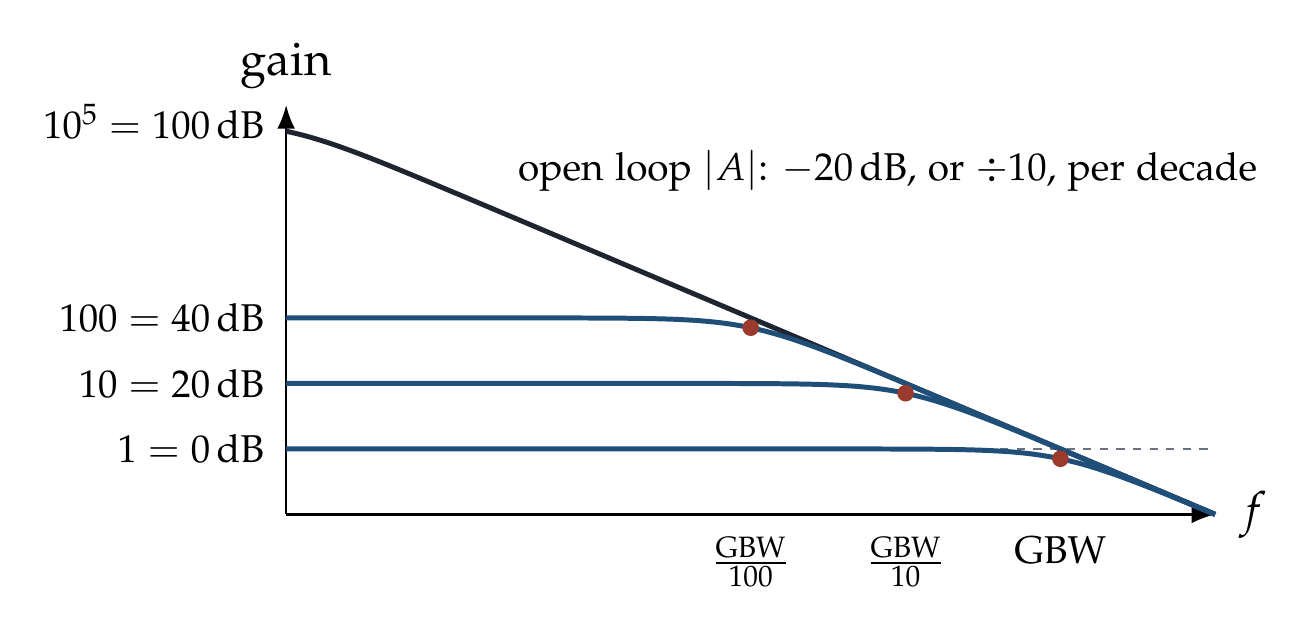
\begin{tikzpicture}
  \begin{semilogxaxis}[bode, width=118mm, height=52mm, xmin=10, xmax=1e7, ymin=-20, ymax=105, domain=10:1e7,
      xtick={1e4,1e5,1e6}, xticklabels={$\tfrac{\text{GBW}}{100}$,$\tfrac{\text{GBW}}{10}$,GBW},
      ytick={0,20,40,100}, yticklabels={$1=0$\,dB,$10=20$\,dB,$100=40$\,dB,$10^5=100$\,dB}, ylabel={gain},
      every axis y label/.style={at={(axis description cs:0,1)}, anchor=south}]
    \draw[muted, dashed, line width=0.8pt] (axis cs:10,0) -- (axis cs:1e7,0);
    \addplot[ink] {100-10*log10(1+(x/10)^2)};
    \addplot[vout] {40-10*log10(1+(x/1e4)^2)};
    \addplot[vout] {20-10*log10(1+(x/1e5)^2)};
    \addplot[vout] {-10*log10(1+(x/1e6)^2)};
    \fill[trap] (axis cs:1e4,37) circle (3pt) (axis cs:1e5,17) circle (3pt) (axis cs:1e6,-3) circle (3pt);
    \node[tag, anchor=west] at (axis cs:300,85) {open loop $|A|$: $-20$\,dB, or $\div10$, per decade};
  \end{semilogxaxis}
  \end{tikzpicture}}
\begin{eqgroup}[The corner sits where the closed loop meets $|A|$]
\[ f_{-3\,\text{dB}}=\frac{\text{GBW}}{1/\beta}\qquad \varepsilon\approx\frac{1/\beta}{|A(f)|} \]
\note{A 1\,MHz part has $|A|=100$ at 10\,kHz: a gain of 10 there is already 9\,\% short.}
\end{eqgroup}
\tcblower
\trap{\textbf{Count the noise gain, not the signal gain:} an inverting $-1$ has half a follower's bandwidth.}
\end{card}
% ---------------------------------------------------------------- slew rate
\begin{card}[height=169mm, valign upper=center]{Slew rate}{The output has a speed limit, in volts per microsecond.}%
  {Large-signal audio, DAC outputs, fast edges into ADCs.}
\wideplot{%
  \begin{tikzpicture}
  \begin{axis}[wave, width=112mm, height=52mm, ymin=-1.3, ymax=1.3]
    \addplot[vin] {sin(x)};
    \addplot[vbad] {0.8*tri(x-18)};
    \node[tag, text=trap, anchor=west] at (axis cs:122,0.2) {slope $=$ SR};
    \node[tag, text=muted, anchor=south] at (axis cs:90,1.02) {asked for};
  \end{axis}
  \end{tikzpicture}}
\begin{eqgroup}[A sine's steepest slope is $2\pi fV_p$]
\[ \text{SR}=\Bigl|\frac{dv_\text{out}}{dt}\Bigr|_\text{max}\qquad f_\text{FP}=\frac{\text{SR}}{2\pi V_p} \]
\note{0.5\,V/\textmu s and 10\,V peaks: full power ends at 8\,kHz, on a 1\,MHz op-amp.}
\end{eqgroup}
\tcblower
\trap{\textbf{A small-signal test hides it.} Bandwidth is measured at 100\,mV; slew only shows at full swing.}
\end{card}
% ---------------------------------------------------------------- phase margin
\begin{card}[height=169mm, valign upper=center]{Phase margin}{Overshoot is the margin you did not keep.}%
  {Followers, TIAs, differentiators, cables and other capacitive loads.}
\figs{%
  % the loop-gain plot of commandment II: L(s) = 1.2256 / (s (1+s/1.5) (1+s/5)), crossover at 1, PM 45 deg,
  % GM 14.5 dB. Gain (left axis) and phase (right axis) share one box with 0 dB level with -180 deg,
  % so both margins are gaps to the same line.
  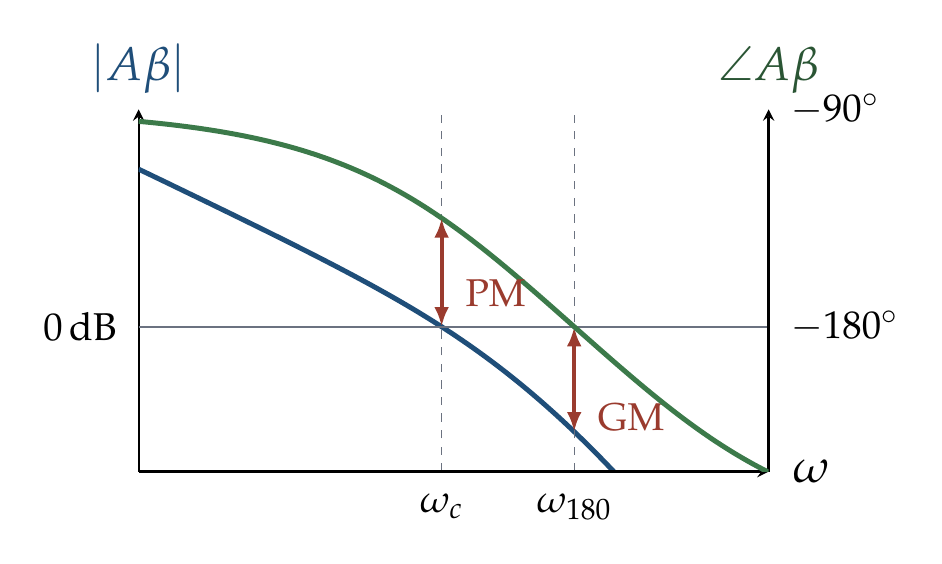
\begin{tikzpicture}
  \pgfplotsset{loopplot/.style={bode, width=80mm, height=46mm, xmin=0.1, xmax=12,
     samples=120, domain=0.1:12, restrict y to domain=-400:400, clip=true}}
  \begin{semilogxaxis}[loopplot, name=mag, axis x line=none, axis y line=left, ymin=-20, ymax=30,
     ylabel={$|A\beta|$}, every axis y label/.style={at={(axis description cs:0,1)}, anchor=south, text=accent},
     ytick={0}, yticklabels={0\,dB}]
    \addplot[accent] {20*log10(1.2256) - 20*log10(x) - 10*log10(1+(x/1.5)^2) - 10*log10(1+(x/5)^2)};
    \draw[muted, line width=0.8pt] (axis cs:0.1,0) -- (axis cs:12,0);
    \draw[muted, dashed, thin] (axis cs:1,-20) -- (axis cs:1,30);
    \draw[muted, dashed, thin] (axis cs:2.739,-20) -- (axis cs:2.739,30);
    \draw[{Latex[length=2.5mm]}-{Latex[length=2.5mm]}, trap, line width=1.4pt] (axis cs:2.739,-14.5) -- (axis cs:2.739,0);
    \node[trap, font=\small, anchor=west] at (axis cs:2.9,-12.5) {GM};
  \end{semilogxaxis}
  \begin{semilogxaxis}[loopplot, at={(mag.south west)}, axis y line=right, axis x line=bottom, ymin=-240, ymax=-90,
     xlabel={$\omega$}, ylabel={$\angle A\beta$},
     every axis y label/.style={at={(axis description cs:1,1)}, anchor=south, text=good!70!black},
     xtick={1,2.739}, xticklabels={$\omega_c$,$\omega_{180}$},
     ytick={-90,-180}, yticklabels={$-90^\circ$,$-180^\circ$}]
    \addplot[good] {-90 - atan(x/1.5) - atan(x/5)};
    \draw[{Latex[length=2.5mm]}-{Latex[length=2.5mm]}, trap, line width=1.4pt] (axis cs:1,-180) -- (axis cs:1,-135);
    \node[trap, font=\small, anchor=west] at (axis cs:1.06,-166) {PM};
  \end{semilogxaxis}
  \end{tikzpicture}}{%
  \begin{tikzpicture}
  \begin{axis}[wave, width=50mm, height=46mm, domain=0:16, xmin=0, xmax=17, ymin=-0.1, ymax=1.8, samples=200]
    \addplot[vin] {x<0.05 ? 0 : 1};
    \addplot[vbad] {stepresp(0.15)};
    \addplot[muted, line width=1.6pt] {stepresp(0.4)};
    \addplot[vout] {stepresp(0.7)};
    \node[tag, text=trap, anchor=south west] at (axis cs:3.3,1.6) {$17^\circ$};
    \node[tag, text=muted, anchor=west] at (axis cs:5.2,1.3) {$43^\circ$};
    \node[tag, text=accent, anchor=north west] at (axis cs:4.6,0.9) {$65^\circ$};
  \end{axis}
  \end{tikzpicture}}
\begin{eqgroup}[Margin $\approx100\,\zeta$ degrees, for $\zeta<0.7$]
\[ \text{PM}=180^\circ+\angle A\beta\,\bigr|_{|A\beta|=1}\qquad \text{OS}=e^{-\pi\zeta/\sqrt{1-\zeta^2}} \]
\note{Where $1/\beta$ meets $|A|$, a closing rate of 20\,dB/dec leaves about $90^\circ$; 40\,dB/dec leaves none.
      A capacitive load adds a pole through $r_o$: isolate it with 10--100\,$\Omega$ in series.}
\end{eqgroup}
\tcblower
\trap{\textbf{Decompensated parts are stable only above a minimum gain.} As followers, they oscillate.}
\end{card}
% ---------------------------------------------------------------- CMRR and PSRR
\begin{card}[height=169mm, valign upper=center]{CMRR and PSRR}{Rejection fades with frequency.}%
  {Switching supplies, differential sensing, battery circuits.}
\wideplot{%
  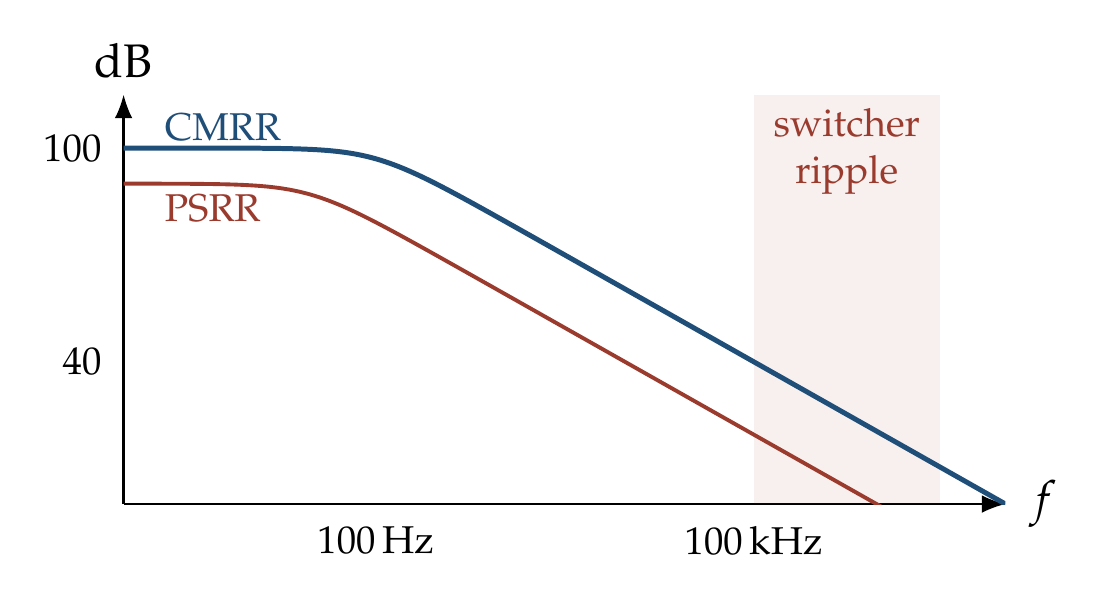
\begin{tikzpicture}
  \begin{semilogxaxis}[bode, width=112mm, height=52mm, xmin=1, xmax=1e7, ymin=0, ymax=115, domain=1:1e7, clip=true,
      xtick={1e2,1e5}, xticklabels={100\,Hz,100\,kHz}, ytick={40,100}, yticklabels={40,100}, ylabel={dB},
      every axis y label/.style={at={(axis description cs:0,1)}, anchor=south}]
    \fill[trap, opacity=0.08] (axis cs:1e5,0) rectangle (axis cs:3e6,115);
    \addplot[vout] {100-10*log10(1+(x/100)^2)};
    \addplot[vbad] {90-10*log10(1+(x/30)^2)};
    \node[tag, text=accent, anchor=south west] at (axis cs:2,101) {CMRR};
    \node[tag, text=trap, anchor=north west] at (axis cs:2,88) {PSRR};
    \node[tag, text=trap, anchor=north, align=center] at (axis cs:5.5e5,112) {switcher\\ ripple};
  \end{semilogxaxis}
  \end{tikzpicture}}
\begin{eqgroup}[Both look like an offset at the input]
\[ \Delta V_{os}=\frac{\Delta v_\text{cm}}{\text{CMRR}}+\frac{\Delta V_S}{\text{PSRR}} \]
\note{Both fall at $-20$\,dB/dec, from the same internal pole as the open-loop gain.}
\end{eqgroup}
\tcblower
\trap{\textbf{100\,dB at DC is 40\,dB at 100\,kHz:} a switching regulator's ripple walks straight in. Filter the rail.}
\end{card}
% ---------------------------------------------------------------- the error budget
\begin{card}[height=169mm, valign upper=center, colframe=ink, colbacktitle=ink]{The error budget}{Everything at the inputs, times the noise gain.}%
  {Precision DC, sensor front ends.}
\begin{eqgroup}[Offsets, bias currents, common mode and supply]
\[ \Delta v_\text{out}=\frac{1}{\beta}\Bigl(V_{os}+I_B\,\Delta R+\frac{v_\text{cm}}{\text{CMRR}}+\frac{\Delta V_S}{\text{PSRR}}\Bigr) \]
\note{$\Delta R$: the difference between the resistances the two inputs see.}
\end{eqgroup}
\begin{eqgroup}[Noise, over the closed-loop bandwidth]
\[ v_{n,\text{out}}=\frac{1}{\beta}\;e_{n,\text{tot}}\sqrt{\tfrac{\pi}{2}\,f_{-3\,\text{dB}}} \]
\end{eqgroup}
\begin{eqgroup}[And the gain itself is short by the loop gain]
\[ \frac{A_\text{cl}}{1/\beta}=\frac{1}{1+1/(A\beta)}\approx1-\frac{1}{A\beta} \]
\note{$A\beta=100$ where you care: 1\,\% gain error, before any resistor tolerance.}
\end{eqgroup}
\tcblower
\trap{\textbf{Add the errors that move together;} root-sum-square the independent ones, and the noise.}
\end{card}
% ---------------------------------------------------------------- offset voltage
\begin{card}[height=169mm, valign upper=center]{Offset voltage}{The inputs never quite agree.}%
  {Thermocouples, strain gauges, integrators, DC-coupled gain.}
\figs{%
  \begin{circuitikz}[sch]
    \node[op amp] (A) at (0,0) {};
    \draw (A.-) -- ++(-0.5,0) coordinate (n);
    \draw (n) to[R, l_=$R_g$, *-] ++(-2,0) -- ++(0,-0.4) node[tground] {};
    \draw (A.+) -- ++(-0.6,0) to[V, l_=$V_{os}$] ++(0,-1.9) node[tground] {};
    \draw (A.out) to[short, -*] ++(0.6,0) coordinate (o) to[short, -o] ++(0.9,0) node[below] {$v_\text{out}$};
    \draw (n) -- ++(0,1.5) coordinate (t) to[R, l=$R_f$] (t -| o) -- (o);
  \end{circuitikz}}{%
  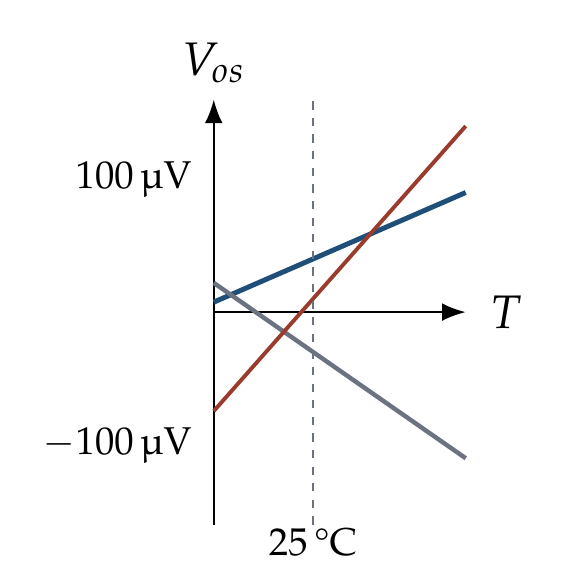
\begin{tikzpicture}
  \begin{axis}[lin, width=32mm, xmin=-40, xmax=125, ymin=-160, ymax=160, domain=-40:125,
      xlabel={$T$}, ylabel={$V_{os}$}, xtick=\empty,
      extra description/.code={\node[tag, anchor=north] at (axis cs:25,-160) {25\,\textdegree C};
        \draw[muted, dashed, thin] (axis cs:25,-160) -- (axis cs:25,160);},
      ytick={-100,100}, yticklabels={$-100$\,\textmu V,$100$\,\textmu V},
      every x tick label/.style={below right}]
    \addplot[vout] {40+0.5*(x-25)};
    \addplot[muted, line width=1.6pt] {-30-0.8*(x-25)};
    \addplot[vbad] {10+1.3*(x-25)};
  \end{axis}
  \end{tikzpicture}}
\begin{eqgroup}[A small battery in series with an input]
\[ \Delta v_\text{out}=\frac{1}{\beta}\,V_{os}\qquad \Delta V_{os}=\text{TC}_{V_{os}}\,\Delta T \]
\note{Every unit has its own $V_{os}$ and its own slope; the datasheet gives the spread.}
\end{eqgroup}
\tcblower
\trap{\textbf{Gain 1000 turns 1\,mV into 1\,V at DC.} Trim it, AC-couple it, or buy zero-drift.}
\end{card}
% ---------------------------------------------------------------- bias current
\begin{card}[height=169mm, valign upper=center]{Bias current}{Rule II leaks.}%
  {pH electrodes, photodiodes, megohm sensors, integrators.}
\figs{%
  \begin{circuitikz}[sch]
    \node[op amp] (A) at (0,0) {};
    \draw (A.-) -- ++(-0.5,0) coordinate (n);
    \draw ($(n)+(-2.1,0)$) node[left] {$v_\text{in}$} to[R, l=$R_\text{in}$, o-*] (n);
    \draw (A.out) to[short, -*] ++(0.6,0) coordinate (o) to[short, -o] ++(0.9,0) node[below] {$v_\text{out}$};
    \draw (n) -- ++(0,1.5) coordinate (t) to[R, l=$R_f$] (t -| o) -- (o);
    \draw (A.+) -- ++(-0.6,0) to[R, l_=$R_c$, fix] ++(0,-1.9) node[tground] {};
  \end{circuitikz}}{%
  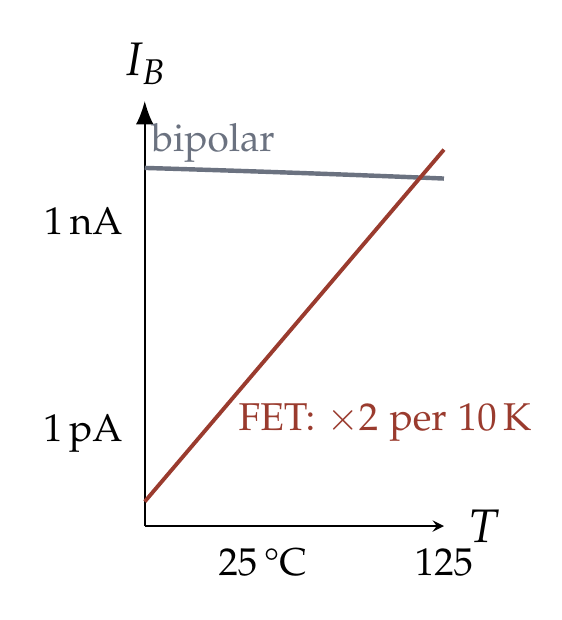
\begin{tikzpicture}
  \begin{semilogyaxis}[lin, axis x line=bottom, xmin=-40, xmax=125, ymin=0.05, ymax=5e4, domain=-40:125,
      xlabel={$T$}, ylabel={$I_B$}, xtick={25,125}, xticklabels={25\,\textdegree C,125},
      ytick={1,1000}, yticklabels={1\,pA,1\,nA},
      every axis x label/.style={at={(axis description cs:1,0)}, anchor=west, xshift=1mm}]
    \addplot[muted, line width=1.6pt] {5000*(1-0.002*(x-25))};
    \addplot[vbad] {10*2^((x-25)/10)};
    \node[tag, text=muted, anchor=south west] at (axis cs:-38,6000) {bipolar};
    \node[tag, text=trap, anchor=north west] at (axis cs:10,3) {FET: $\times2$ per 10\,K};
  \end{semilogyaxis}
  \end{tikzpicture}}
\begin{eqgroup}[$R_c=R_\text{in}\,\|\,R_f$ makes both inputs see the same]
\[ \Delta v_\text{out}=I_B\,R_f\ \xrightarrow{\ R_c\ }\ I_{os}\,R_f \]
\note{$I_{os}$, the mismatch between the two bias currents, is often a tenth of $I_B$.}
\end{eqgroup}
\tcblower
\trap{\textbf{A FET input's picoamps at 25\,\textdegree C are nanoamps at 125\,\textdegree C.} Specify it hot.}
\end{card}
% ---------------------------------------------------------------- noise
\begin{card}[height=169mm, valign upper=center]{Noise}{It is rarely the op-amp: the resistors hiss.}%
  {Microphone, sensor and audio preamps; ADC front ends.}
\figs{%
  % the noise model: a noiseless op-amp, with every source of noise drawn outside it
  \begin{circuitikz}[sch]
    \node[op amp, noinv input up] (A) at (0,0) {};
    \draw (A.+) -- ++(-1.2,0) coordinate (p);
    \draw (p) to[V, l_=$e_n$, color=accent, *-] ++(-2.2,0) coordinate (q);
    \draw (q) to[V, l_=$\sqrt{4kTR_s}$, color=trap] ++(0,-2.2) to[R, l_=$R_s$] ++(0,-1.9) node[tground] {};
    \draw (p) to[I, l_=$i_n$, color=accent] ++(0,-2.6) node[tground] {};
    \draw (A.-) -- ++(-0.3,0);
    \draw (A.out) to[short, -o] ++(0.8,0);
    \node[font=\small, text=muted] at ($(A)+(0.3,-1.6)$) {noiseless};
  \end{circuitikz}}{%
  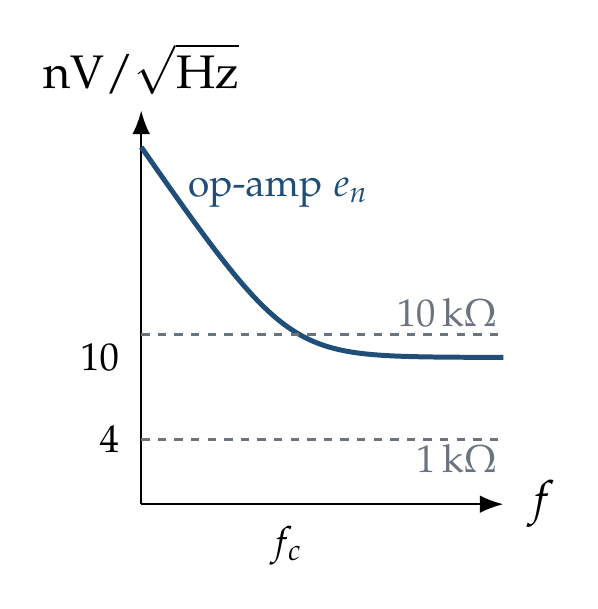
\begin{tikzpicture}
  \begin{loglogaxis}[bode, width=46mm, height=50mm, xmin=1, xmax=1e5, ymin=2, ymax=150, domain=1:1e5,
      xtick={100}, xticklabels={$f_c$}, ytick={4.07,10}, yticklabels={4,10}, ylabel={nV$/\sqrt{\text{Hz}}$},
      every axis y label/.style={at={(axis description cs:0,1)}, anchor=south}]
    \addplot[vout] {10*sqrt(1+100/x)};
    \draw[muted, dashed, line width=1.2pt] (axis cs:1,4.07) -- (axis cs:1e5,4.07);
    \draw[muted, dashed, line width=1.2pt] (axis cs:1,12.9) -- (axis cs:1e5,12.9);
    \node[tag, text=accent, anchor=south west] at (axis cs:4,50) {op-amp $e_n$};
    \node[tag, text=muted, anchor=north east] at (axis cs:9e4,4) {1\,k$\Omega$};
    \node[tag, text=muted, anchor=south east] at (axis cs:9e4,13.5) {10\,k$\Omega$};
  \end{loglogaxis}
  \end{tikzpicture}}
\begin{eqgroup}[Voltage noise, current noise through $R_s$, and $R_s$ itself]
\[ e_{n,\text{tot}}=\sqrt{e_n^2+(i_nR_s)^2+4kTR_s} \]
\note{Every resistor hisses $\sqrt{4kTR}$, the feedback network too: 1\,k$\Omega$ makes 4\,nV$/\sqrt{\text{Hz}}$, as much as a good
      bipolar op-amp. Lower the impedances before you buy a quieter part.}
\end{eqgroup}
\tcblower
\trap{\textbf{Low-$e_n$ bipolar parts have high $i_n$:} above about 10\,k$\Omega$ of source, a FET input is quieter.}
\end{card}
% ---------------------------------------------------------------- chopper
\begin{card}[height=169mm, valign upper=center, colframe=good, colbacktitle=good]{Chopper}{Move the offset to where a filter can remove it.}%
  {Thermocouples, strain gauges, current shunts, weigh scales.}
\figs{%
  % no standard symbol exists; datasheets draw the block diagram, which is the equation below:
  % chop, add the offset, amplify, chop back, filter
  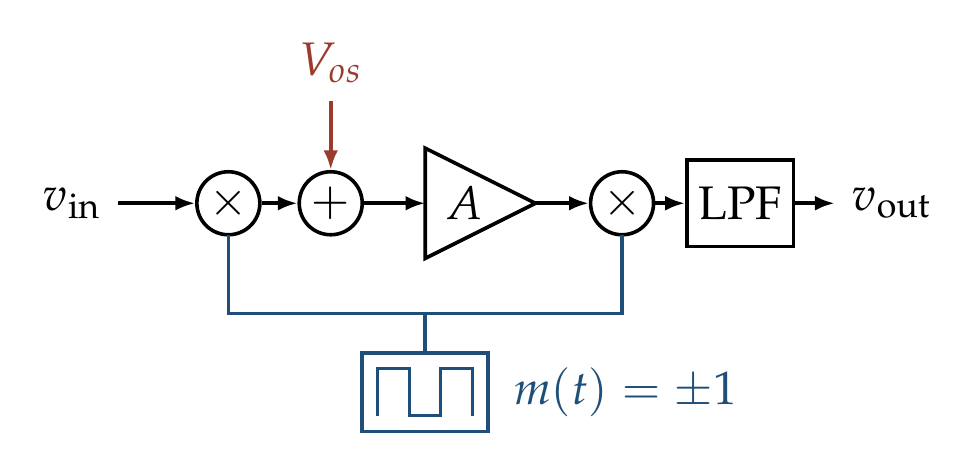
\begin{tikzpicture}[x=1mm, y=1mm, line width=1.3pt, font=\normalsize,
      mix/.style={draw, circle, minimum size=8mm, inner sep=0pt, fill=white},
      blk/.style={draw, minimum height=11mm, inner sep=1.5mm, fill=white}]
    \node[left] (in) at (0,0) {$v_\text{in}$};
    \node[mix] (m1) at (14,0) {$\times$};
    \node[mix] (s) at (27,0) {$+$};
    \draw (39,-7) -- (39,7) -- (53,0) -- cycle; \node at (44,0) {$A$};
    \node[mix] (m2) at (64,0) {$\times$};
    \node[blk] (lp) at (79,0) {LPF};
    \node[right] (out) at (91,0) {$v_\text{out}$};
    \draw[-{Latex[length=2.5mm]}] (0,0) -- (m1);
    \draw[-{Latex[length=2.5mm]}] (m1) -- (s);
    \draw[-{Latex[length=2.5mm]}] (s) -- (39,0);
    \draw[-{Latex[length=2.5mm]}] (53,0) -- (m2);
    \draw[-{Latex[length=2.5mm]}] (m2) -- (lp);
    \draw[-{Latex[length=2.5mm]}] (lp) -- (91,0);
    \draw[vbad, -{Latex[length=2.5mm]}] (27,13) node[above, text=trap] {$V_{os}$} -- (s);
    % the chopping clock, a square wave m(t) = +-1, drives both mixers
    \draw[accent] (14,-4) -- (14,-14) -| (64,-4);
    \draw[accent] (39,-14) -- (39,-19);
    \draw[accent, fill=white] (31,-19) rectangle (47,-29);
    \draw[accent, line width=1.1pt] (33,-27) -- (33,-21) -- (37,-21) -- (37,-27) -- (41,-27) -- (41,-21) -- (45,-21) -- (45,-27);
    \node[text=accent, anchor=west] at (48,-24) {$m(t)=\pm1$};
  \end{tikzpicture}}{%
  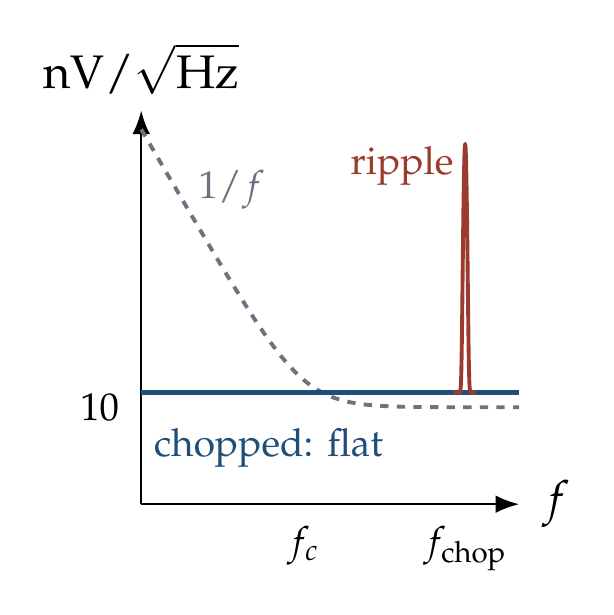
\begin{tikzpicture}
  \begin{loglogaxis}[bode, width=48mm, height=50mm, xmin=0.1, xmax=1e6, ymin=3, ymax=400, domain=0.1:1e6, samples=400,
      xtick={1e2,1e5}, xticklabels={$f_c$,$f_\text{chop}$}, ytick={10}, yticklabels={10}, ylabel={nV$/\sqrt{\text{Hz}}$},
      every axis y label/.style={at={(axis description cs:0,1)}, anchor=south}]
    \addplot[vin] {10*sqrt(1+100/x)};
    \addplot[vout] {12};
    \addplot[vbad, domain=6e4:1.6e5] {12+250*exp(-(ln(x/1e5)/0.08)^2)};
    \node[tag, text=muted, anchor=west] at (axis cs:1,150) {$1/f$};
    \node[tag, text=accent, anchor=north west] at (axis cs:0.15,8) {chopped: flat};
    \node[tag, text=trap, anchor=east] at (axis cs:7e4,200) {ripple};
  \end{loglogaxis}
  \end{tikzpicture}}
\begin{eqgroup}[Swap the inputs with $m(t)=\pm1$, and swap back after the gain]
\[ v_\text{out}=A\,m\bigl(m\,v_\text{in}+V_{os}\bigr)=A\bigl(v_\text{in}+m\,V_{os}\bigr) \]
\note{The signal is chopped twice and comes back; the offset and its $1/f$ noise are chopped once and land at $f_\text{chop}$.}
\note{\tikz[baseline=-0.6ex, x=1mm, y=1mm, line width=1pt, draw=ink]{%
        \draw (0,4) -- (6,2.29) -- (6,-2.29) -- (0,-4) -- cycle;
        \draw (8,1.71) -- (14,0) -- (8,-1.71) -- cycle;
        \draw (6.6,-5) -- (6.6,5) (7.4,-5) -- (7.4,5);}\enspace
      The same trick across a transformer or capacitor barrier is the isolation amplifier; a chopper itself is not isolated.}
\end{eqgroup}
\tcblower
\trap{\textbf{What is left lives at $f_\text{chop}$:} ripple, intermodulation, and bias-current spikes. Keep the signal well below it.}
\end{card}
% ---------------------------------------------------------------- input stage
\begin{card}[height=169mm, valign upper=center, colframe=ink, colbacktitle=ink]{Input stage}{Pick it by the source impedance.}%
  {Choosing a part.}
\begin{eqgroup}[Orders of magnitude, at room temperature]
{\small\centering\renewcommand{\arraystretch}{1.35}%
\begin{tabular}{@{}l@{\hspace{4mm}}c@{\hspace{4mm}}c@{\hspace{4mm}}c@{\hspace{4mm}}c@{}}
                  & \bfseries bipolar & \bfseries JFET & \bfseries CMOS & \bfseries zero-drift \\
  $V_{os}$         & 10--100\,\textmu V & 0.1--2\,mV & 0.1--5\,mV & 1--10\,\textmu V \\
  drift, per K    & 0.1--1\,\textmu V & 2--10\,\textmu V & 1--5\,\textmu V & 10--50\,nV \\
  $I_B$           & 1--50\,nA & 1--50\,pA & 1\,pA & 0.1--1\,nA \\
  $e_n$, nV$/\sqrt{\text{Hz}}$ & 1--10 & 5--20 & 10--50 & 10--60 \\
  $i_n$           & pA$/\sqrt{\text{Hz}}$ & fA$/\sqrt{\text{Hz}}$ & fA$/\sqrt{\text{Hz}}$ & pA$/\sqrt{\text{Hz}}$ \\
  \itshape for    & \itshape low-ohm & \itshape high-ohm & \itshape low power & \itshape DC precision \\
\end{tabular}\par}
\end{eqgroup}
\begin{eqgroup}[Where voltage noise and current noise break even]
\[ R_{s,\text{opt}}=\frac{e_n}{i_n} \]
\note{Bipolar: kilohms. FET: megohms and up. Zero-drift chops away the $1/f$ noise and the drift.}
\end{eqgroup}
\tcblower
\trap{\textbf{Design with the max column, hot,} not the typical one at 25\,\textdegree C.}
\end{card}
% ---------------------------------------------------------------- output swing
\begin{card}[height=169mm, valign upper=center]{Output swing}{Rail-to-rail means tens of millivolts short.}%
  {Single-supply and battery circuits, ADC drivers.}
\wideplot{%
  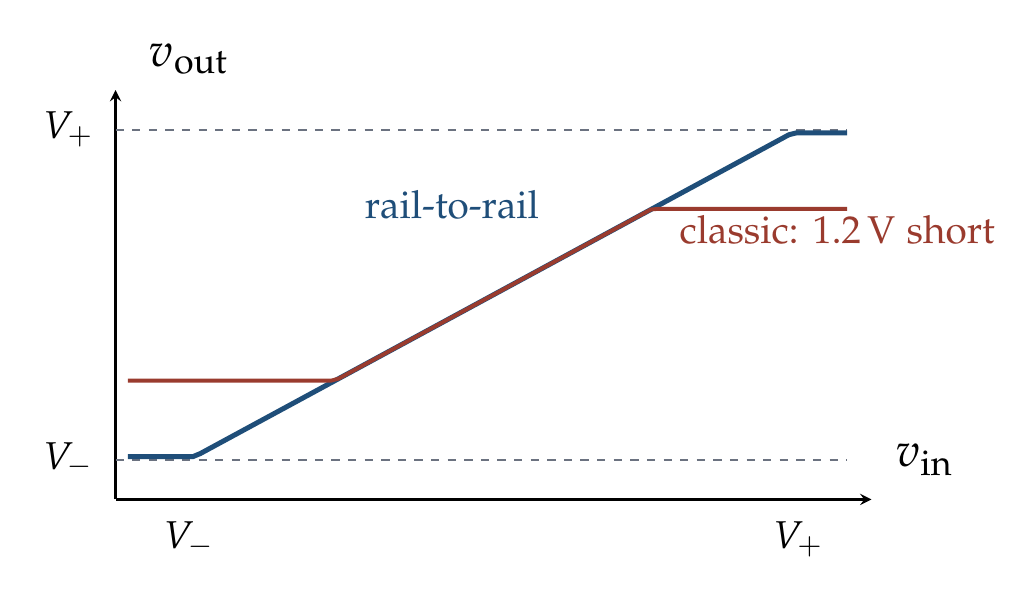
\begin{tikzpicture}
  \begin{axis}[xfer, width=96mm, height=52mm, xmin=-0.6, xmax=5.6, ymin=-0.6, ymax=5.6, domain=-0.5:5.4, samples=100,
      xtick={0,5}, xticklabels={$V_-$,$V_+$}, ytick={0,5}, yticklabels={$V_-$,$V_+$}, axis lines=left]
    \draw[muted, dashed, line width=0.8pt] (axis cs:-0.6,5) -- (axis cs:5.4,5) (axis cs:-0.6,0) -- (axis cs:5.4,0);
    \addplot[vout] {min(max(x,0.05),4.95)};
    \addplot[vbad] {min(max(x,1.2),3.8)};
    \node[tag, text=accent, anchor=south east] at (axis cs:2.9,3.6) {rail-to-rail};
    \node[tag, text=trap, anchor=north west] at (axis cs:4,3.75) {classic: 1.2\,V short};
  \end{axis}
  \end{tikzpicture}}
\begin{eqgroup}[The output transistors need headroom, more as the load pulls]
\[ V_-+V_{OL}\ \le\ v_\text{out}\ \le\ V_+-V_{OH} \]
\note{$V_{OH}$ and $V_{OL}$: 1--2\,V for classic outputs, 10--100\,mV for rail-to-rail, both growing with load current.}
\end{eqgroup}
\tcblower
\trap{\textbf{A single-supply output never reaches 0\,V.} The ADC's ``zero'' is tens of millivolts.}
\end{card}
% ---------------------------------------------------------------- input range
\begin{card}[height=169mm, valign upper=center]{Input range}{Rule I needs the inputs inside their range.}%
  {Followers and non-inverting stages on a single supply.}
\wideplot{%
  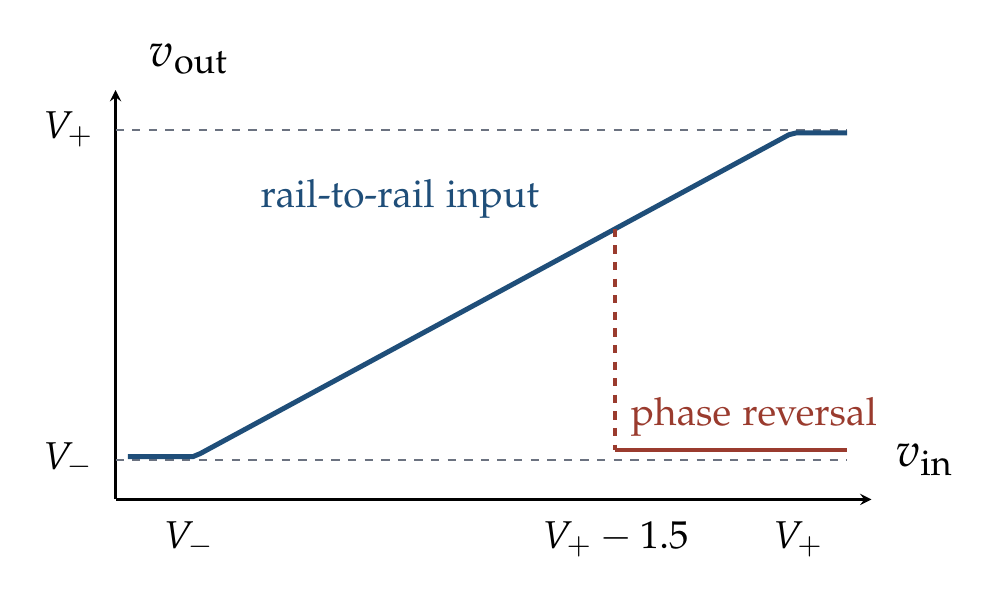
\begin{tikzpicture}
  \begin{axis}[xfer, width=96mm, height=52mm, xmin=-0.6, xmax=5.6, ymin=-0.6, ymax=5.6, domain=-0.5:5.4, samples=100,
      xtick={0,3.5,5}, xticklabels={$V_-$,$V_+-1.5$,$V_+$}, ytick={0,5}, yticklabels={$V_-$,$V_+$}, axis lines=left]
    \draw[muted, dashed, line width=0.8pt] (axis cs:-0.6,5) -- (axis cs:5.4,5) (axis cs:-0.6,0) -- (axis cs:5.4,0);
    \addplot[vout] {min(max(x,0.05),4.95)};
    \addplot[vbad, domain=3.5:5.4] {0.15};
    \draw[vbad, dashed] (axis cs:3.5,3.5) -- (axis cs:3.5,0.15);
    \node[tag, text=accent, anchor=south east] at (axis cs:2.9,3.6) {rail-to-rail input};
    \node[tag, text=trap, anchor=south west] at (axis cs:3.6,0.3) {phase reversal};
  \end{axis}
  \end{tikzpicture}}
\begin{eqgroup}[A follower's input common-mode range, classic part]
\[ V_-\ \le\ v_\text{cm}\ \le\ V_+-1.5\,\text{V} \]
\note{Rail-to-rail inputs use two input pairs; where they hand over, the offset steps by up to a millivolt.}
\end{eqgroup}
\tcblower
\trap{\textbf{Beyond its range, some parts invert the output.} A servo loop then runs away at full speed.}
\end{card}
% ---------------------------------------------------------------- input protection
\begin{card}[height=169mm, valign upper=center]{Input protection}{Absolute maximum: the inputs stay inside the rails.}%
  {Connectors, long sensor cables, anything hot-plugged.}
\figs{%
  \begin{circuitikz}[sch]
    \node[op amp, noinv input up] (A) at (0,0) {};
    \draw (A.+) -- ++(-1.1,0) coordinate (p);
    \draw ($(p)+(-1.8,0)$) node[left] {$v_\text{in}$} to[R, l=$R_s$, fix, o-*] (p);
    \draw (p) to[D, fix] ++(0,1.5) node[above] {$V_+$};
    \draw ($(p)+(0,-1.5)$) node[below] {$V_-$} to[D, fix] (p);
    \draw (A.out) to[short, -*] ++(0.5,0) coordinate (o) to[short, -o] ++(0.8,0) node[above] {$v_\text{out}$};
    \draw (A.-) -- ++(-0.5,0) |- ($(o)+(0,-2)$) -- (o);
  \end{circuitikz}}{%
  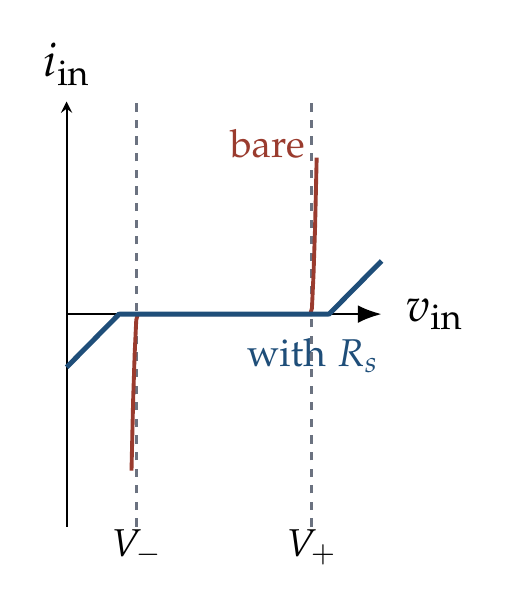
\begin{tikzpicture}
  \begin{axis}[xfer, width=40mm, xmin=-2, xmax=7, ymin=-3, ymax=3, domain=-2:7, samples=200, restrict y to domain=-3:3,
      axis y line=left, every axis y label/.style={at={(axis description cs:0,1)}, anchor=south},
      ylabel={$i_\text{in}$}, xtick=\empty, ytick=\empty]
    \draw[muted, dashed, line width=0.8pt] (axis cs:0,-3) -- (axis cs:0,3) (axis cs:5,-3) -- (axis cs:5,3);
    \node[tag, anchor=north] at (axis cs:0,-3) {$V_-$};
    \node[tag, anchor=north] at (axis cs:5,-3) {$V_+$};
    \addplot[vbad] {x>5 ? exp(8*(x-5))-1 : (x<0 ? 1-exp(-8*x) : 0)};
    \addplot[vout] {x>5.5 ? 0.5*(x-5.5) : (x<-0.5 ? 0.5*(x+0.5) : 0)};
    \node[tag, text=trap, anchor=east] at (axis cs:4.9,2.4) {bare};
    \node[tag, text=accent, anchor=north east] at (axis cs:7,-0.3) {with $R_s$};
  \end{axis}
  \end{tikzpicture}}
\begin{eqgroup}[Limit the current the ESD diodes must carry]
\[ R_s\ \ge\ \frac{v_\text{in,max}-V_S}{10\,\text{mA}} \]
\note{Many bipolar parts clamp $|v_+-v_-|$ to 0.7\,V with diodes: they cannot be used as comparators.}
\end{eqgroup}
\tcblower
\trap{\textbf{A signal with the supply off powers the chip through its ESD diodes,} or latches it up.}
\end{card}
% ---------------------------------------------------------------- decoupling
\begin{card}[height=169mm, valign upper=center]{Decoupling}{The supply pins are inputs too.}%
  {Every board; fast op-amps first.}
\figs{%
  \begin{circuitikz}[sch]
    \node[op amp] (A) at (0,0) {};
    \draw (A.-) to[short, -o] ++(-1,0);
    \draw (A.+) to[short, -o] ++(-1,0);
    \draw (A.out) to[short, -o] ++(1,0);
    \draw (A.up) -- ++(0,0.9) coordinate (vp) to[short, -o] ++(-1.6,0) node[left] {$V_+$};
    \draw (A.down) -- ++(0,-0.9) coordinate (vm) to[short, -o] ++(-1.6,0) node[left] {$V_-$};
    \draw (vp) to[C, l=100\,nF, fix, *-] ++(2.2,0) node[tground] {};
    \draw (vm) to[C, l_=100\,nF, fix, *-] ++(2.2,0) node[tground] {};
  \end{circuitikz}}{%
  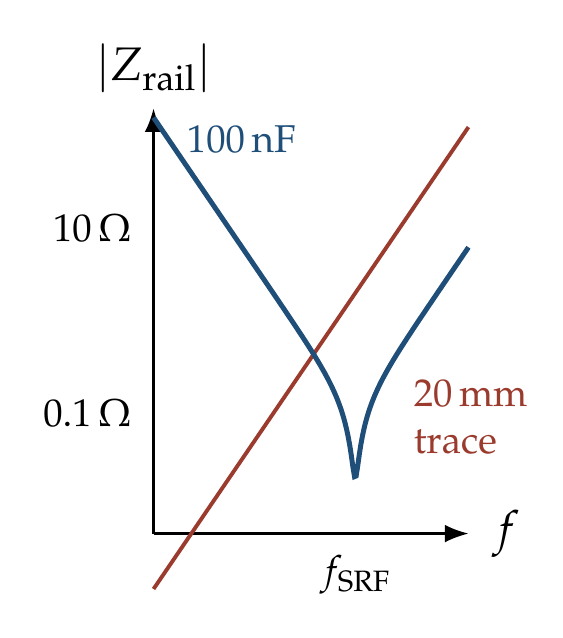
\begin{tikzpicture}
  \begin{loglogaxis}[bode, width=40mm, xmin=1e4, xmax=1e9, ymin=0.005, ymax=200, domain=1e4:1e9,
      xtick={1.6e7}, xticklabels={$f_\text{SRF}$}, ytick={0.1,10}, yticklabels={0.1\,$\Omega$,10\,$\Omega$},
      ylabel={$|Z_\text{rail}|$}, every axis y label/.style={at={(axis description cs:0,1)}, anchor=south}]
    \addplot[vbad] {2*pi*x*2e-8};
    \addplot[vout] {sqrt(0.02^2+(2*pi*x*1e-9-1/(2*pi*x*1e-7))^2)};
    \node[tag, text=trap, anchor=north west, align=left] at (axis cs:1.2e8,0.25) {20\,mm\\ trace};
    \node[tag, text=accent, anchor=south west] at (axis cs:3e4,60) {100\,nF};
  \end{loglogaxis}
  \end{tikzpicture}}
\begin{eqgroup}[A trace is an inductor, about 1\,nH per millimetre]
\[ f_\text{SRF}=\frac{1}{2\pi\sqrt{L_\text{ESL}\,C}} \]
\note{100\,nF within a few millimetres of each supply pin, returned straight to the ground plane; 10\,\textmu F per rail nearby.}
\end{eqgroup}
\tcblower
\trap{\textbf{Without local decoupling, the supply trace sits inside the loop:} fast op-amps oscillate.}
\end{card}
\end{tcbraster}
\end{minipage}
\end{document}
